\documentclass[a4paper,8pt]{beamer}
\usepackage[slovene]{babel}
\usepackage[utf8]{inputenc}
\usepackage[T1]{fontenc}
\usepackage{lmodern}
\usepackage{amsmath}
\usepackage{array}
\usepackage{tikz}

%\setbeamertemplate{navigation symbols}{}

\usetheme{Berlin}
\beamertemplatenavigationsymbolsempty
\setbeamertemplate{headline}{}
\usecolortheme{default}
\useinnertheme{rounded}
\useoutertheme{infolines}

\usepackage{palatino}
\usefonttheme{serif}

\setbeamertemplate{navigation symbols}{}

\usepackage{subfig}
\usepackage{graphicx}
\graphicspath{{./slike/}}


\newcommand{\R}{\mathbb R}
\newcommand{\N}{\mathbb N}
\newcommand{\Z}{\mathbb Z}

\newtheorem{definicija}{Definicija}
\newtheorem{izrek}{Izrek}
\newtheorem{lema}{Lema}
\newtheorem{trditev}{Trditev}
\newtheorem{posledica}{Posledica}
\newtheorem{primer}{Primer}

\newcommand{\tbf}{\textbf}

\title{Gregoryjeve krpe}
\author{Klara Kresnik in Meta Trdin} % \\ ndlkndl}
%\author[My name]{\textbf {Directed by: my name\\ \footnotesize Supervised by: first name, second name}}
\institute[FMF]{Fakulteta za matematiko in fiziko}
\date{}




\begin{document}

\begin{frame}
\maketitle
\end{frame}

\begin{frame}{Vsebina}

% da bo na tem slajdu pisava večja
\fontsize{14pt}{7.2}\selectfont

\begin{enumerate}
	\item Uvod
	\item Metoda Chiyokura in Kimura
	\item Gregoryjeve krpe
	\begin{itemize}
		\fontsize{10pt}{7.2}\selectfont
		\item Kvadratne Gregoryjeve krpe
		\item Trikotne Gregoryjeve krpe
	\end{itemize}
    \item Primeri
\end{enumerate}

\end{frame}

\section{Uvod}
\begin{frame}{Uvod}
\begin{itemize}
	\item Naloga: Zlepiti krpe oziroma ploskve tako, da bo imel zlepek geometrijsko zveznost reda 1. 
	\item Uporaba: pri geometrijskem modeliranju in v računalniški 	grafiki
	
	\item Vemo: $G^1 \leftrightarrow$ zveznost enotskih tangent
	\item Ko združujemo dve krpi, nastane problem - twist compatibility problem
	\pause
	\begin{figure}[h]
		\centering
		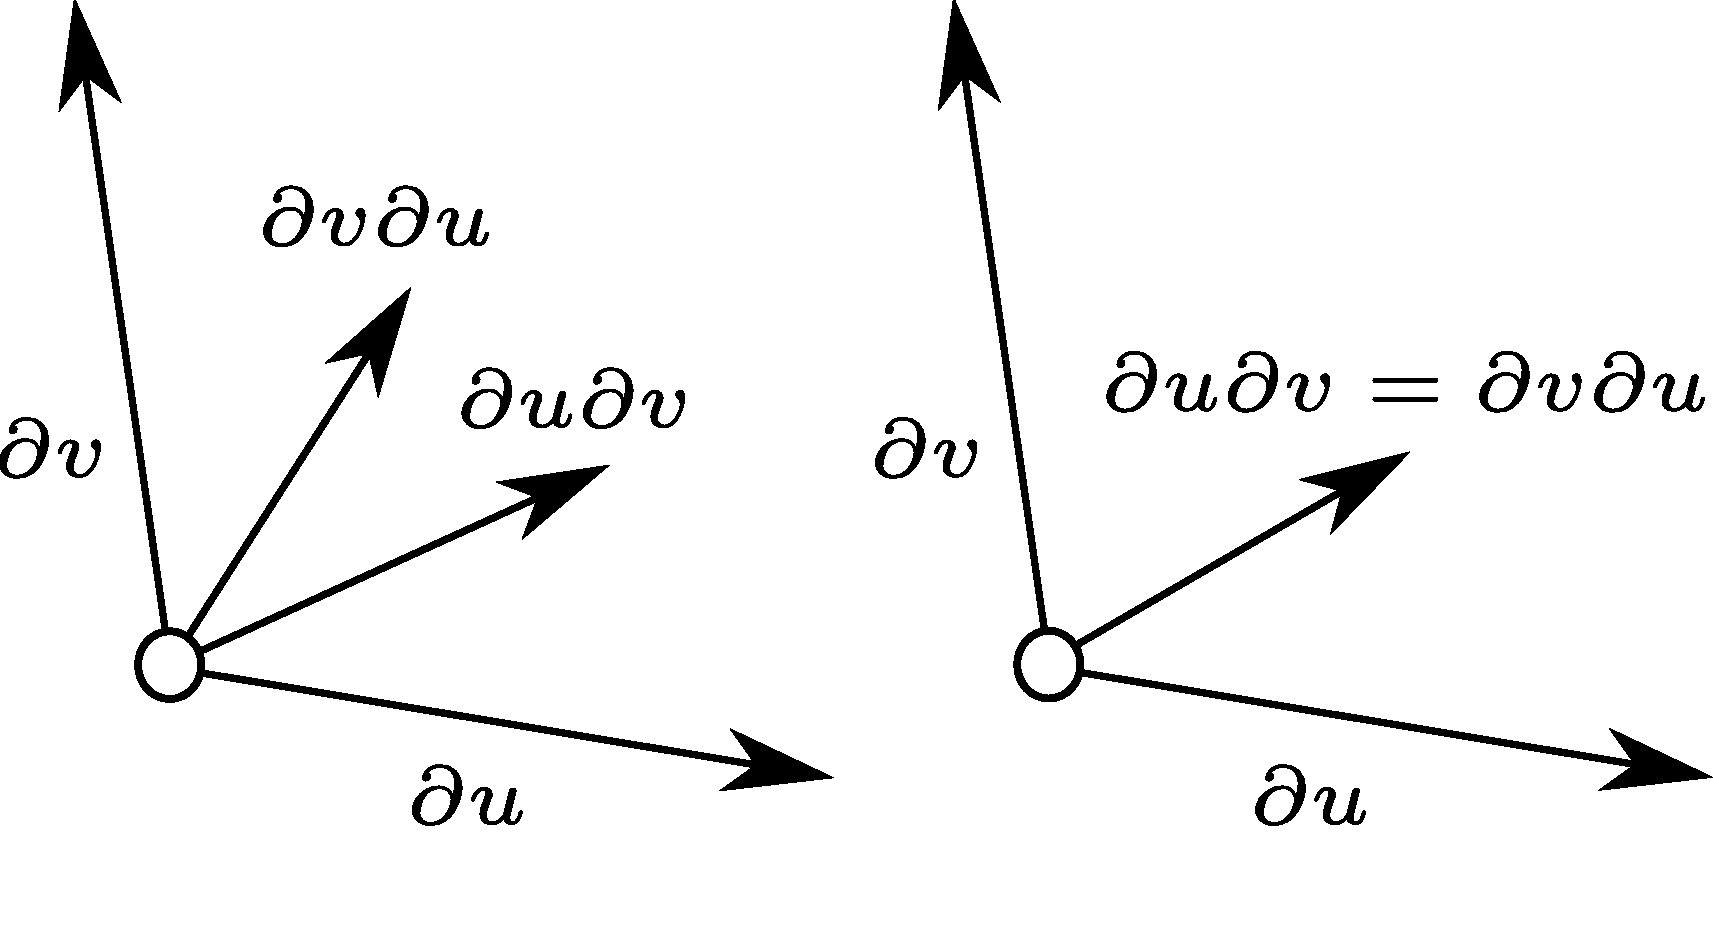
\includegraphics[width=4cm]{mesani_odvodi_ob.jpg}
		%\caption{Mešani odvodi}
	\end{figure}
	Mešani odvodi se ne rabijo nuno ujemati. $\rightarrow$ Prednost Gregoryjevih krp. To se pokaže v notranjih kontrolnih točkah, ki bodo kar funkcije. Ploskev bo sama po sebi racionalna.
	%\item Rešitev: Uporabimo racionalne funkcije, ki mešane odvode primerno zrdužijo.
	\item Podano: robne krivulje. Dobiti želimo notranje kontrolne točke. Potrebovali bomo tudi podatke iz tangentne ravnine na robu.

	
\end{itemize}

\end{frame}

\section{Metoda Chiyokura in Kimura}
\begin{frame}{Metoda Chiyokura in Kimura}
	\begin{itemize}
		\item <1->Metoda združi dve Bézierjevi krpi, tako da je zlepek na robu $G^1$ zvezen, zgolj s podatki
		o robni krivulji in pripadajoči tangenti ravnini.
		\item <1-> Vsaka robna krivulja je definirana s kontrolnim poligonom.
	\end{itemize}

	\uncover<2->{
		\[
			\text{det} ( \partial \Gamma (u), \partial \Gamma_a (u), \partial \Gamma_b (u)) = 0 
		\]
	}

	\uncover<3->{
		\[
			\partial \Gamma (u) = k(u) \partial \Gamma_a (u) + h(u) \partial \Gamma_b (u)
		\]
	}
	
\end{frame}

\begin{frame}{Metoda Chiyokura in Kimura}
	\begin{columns}
		\begin{column}{0.45\textwidth}
			\begin{figure}[h]
				\centering
				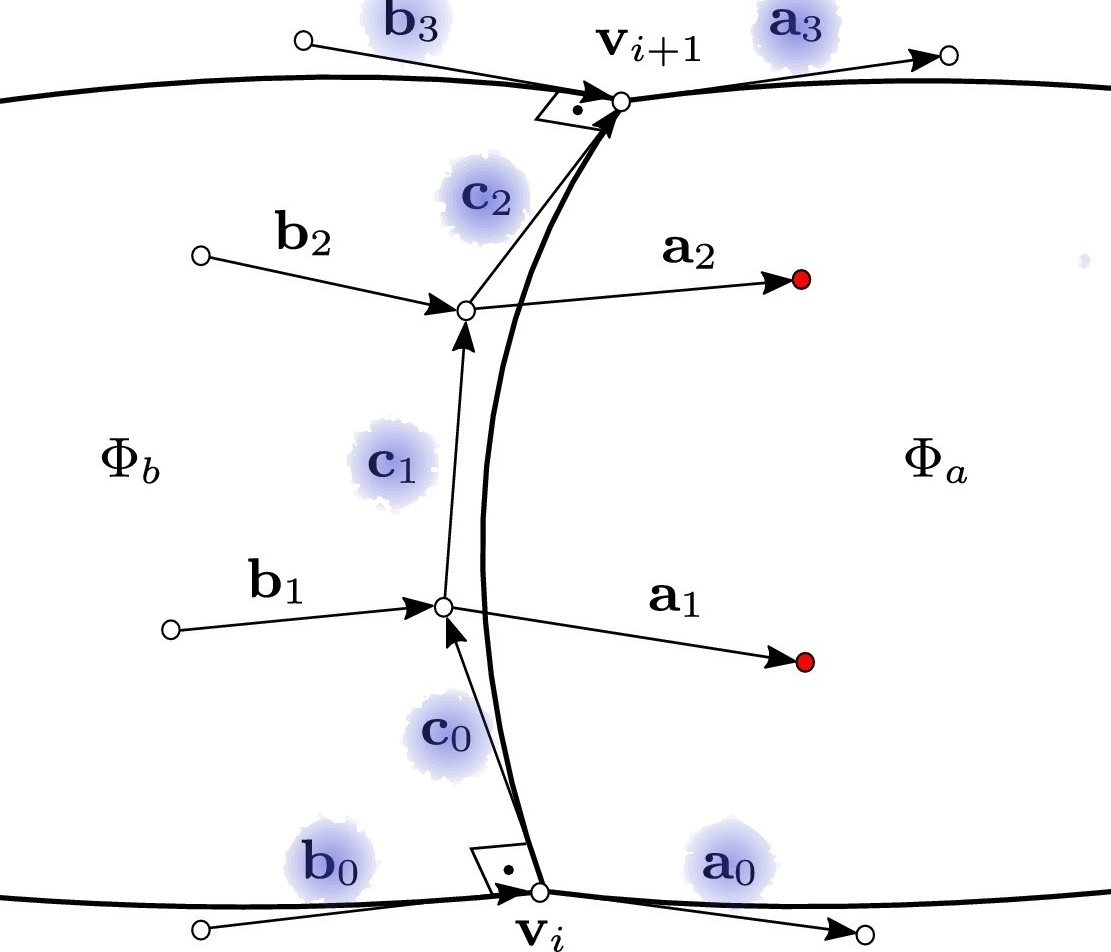
\includegraphics[width=6cm]{metoda_CinK_pobarvano.jpg}
				\caption{Metoda Chiyokura in Kimura}
			\end{figure}
		\end{column}

		\begin{column}{0.55\textwidth}
			\uncover<2->{
				\begin{equation*}
					\begin{split}
						\tbf{a}_0 &= k_0\tbf{b}_0 + h_0\tbf{c}_0 \\
						\tbf{b}_1 &= \frac{2}{3}\tbf{b}_0 + \frac{1}{3}\tbf{b}_3
					\end{split}
					\quad\quad
					\begin{split}
						\tbf{a}_3 &= k_1\tbf{b}_3 + h_1\tbf{c}_2 \\
						\tbf{b}_2 &= \frac{1}{3}\tbf{b}_0 + \frac{2}{3}\tbf{b}_3
					\end{split}
				\end{equation*}
			}

			\uncover<3->{
				\begin{align*}
					\tbf{a}_1 &= (k_1 - k_0)\frac{\tbf{b}_0}{3} + k_0\tbf{b}_1 + 2h_0\frac{\tbf{c}_1}{3} + h_1\frac{\tbf{c}_0}{3} \\
					\tbf{a}_2 &= k_1\tbf{b}_2 - (k_1 - k_0)\frac{\tbf{b}_3}{3} + h_0\frac{\tbf{c}_2}{3} + 2h_1\frac{\tbf{c}_1}{3}
				\end{align*}
			}
		\end{column}
	\end{columns}
	
\end{frame}


\section{Gregoryjeve krpe}
\begin{frame}{Kvadratne Gregoryjeve krpe}


Konstrukcija
\begin{itemize}
	%\item Želimo parametrizirati ploskev v prostoru, da bo imela $G^1$ zveznost, ko jo bomo zlepili.
	\item Domena $[0,1] \times [0,1]$
	\item Podane imamo $4$ robne krivulje: Bézierjeve krivulje reda $3$
	\item Na vsakem robu uporabimo metodo Chiyokura in Kimura (dobimo $2 \cdot 4 = 8$ točk)
	\item Nastopi twist compatibility problem. Tukaj si pomagamo z racionalnimi funkcijami:
		\begin{align*}
		\tbf{b}_{11} (u, v) &=  \frac{v \textbf{b}_{11,u_0}+u\tbf{b}_{11,v_0}}{u +v} \\
		\tbf{b}_{21} (u, v) &= \frac{(1-v) \tbf{b}_{21,u_0}+u\tbf{b}_{21,v_1}}{(1-v)+u} \\
		\tbf{b}_{12} (u, v) &= \frac{v \tbf{b}_{12,u_1}+(1-u)\tbf{b}_{12,v_0}}{v+(1-u)} \\
		\tbf{b}_{22} (u, v) &= \frac{(1-v) \tbf{b}_{22,u_1}+(1-u)\tbf{b}_{22,v_1}}{(1-u)+(1-v)} 
		\end{align*}
\end{itemize}
	
\end{frame}
\begin{frame}
	\begin{figure}[h]
		\centering
		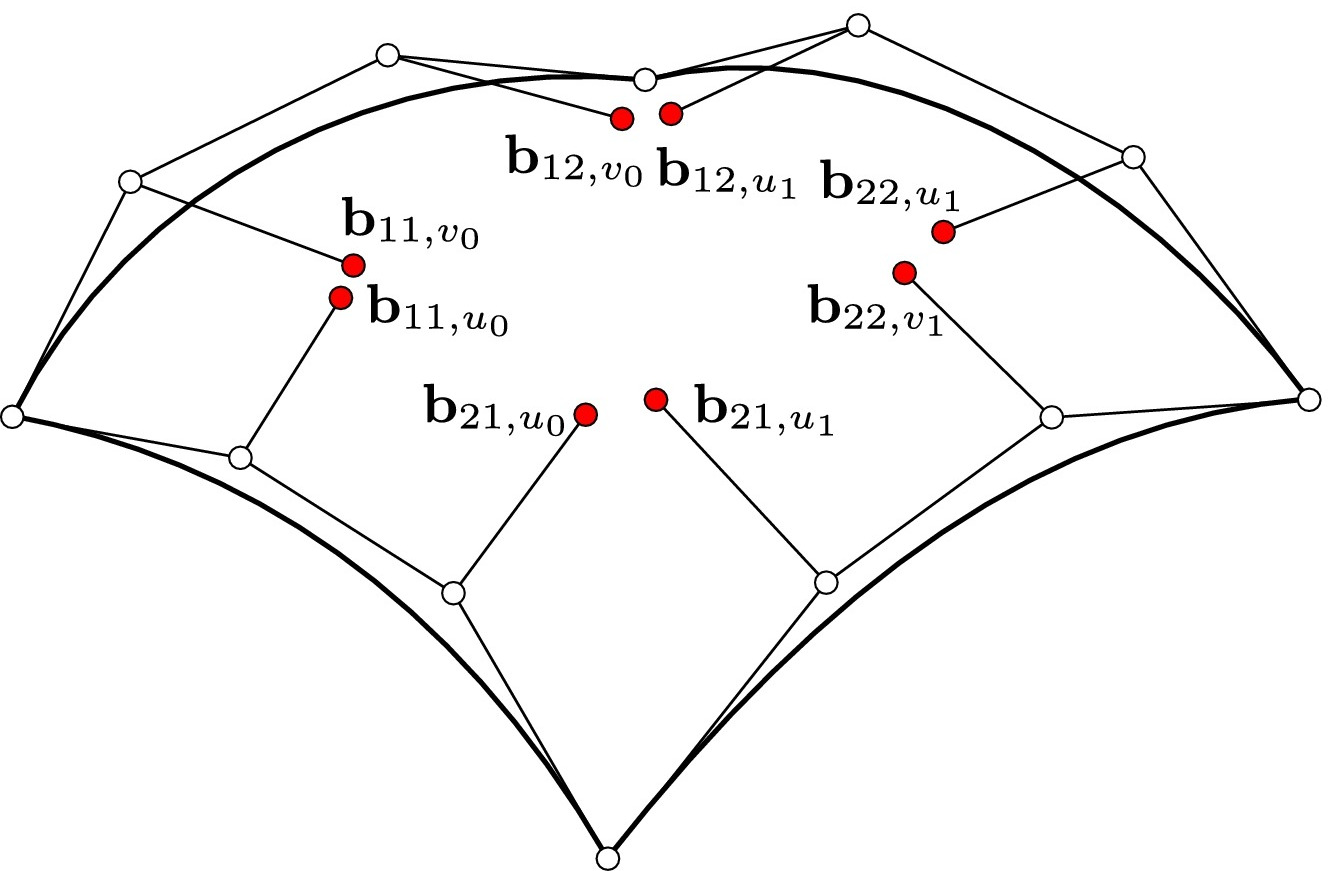
\includegraphics[width=10cm]{gregory_krpe_kvadratna.jpg}
		\caption{Kvadratna Gregoryjeva krpa}
	\end{figure}
\end{frame}

\begin{frame}{Trikotne Gregoryjeve krpe}
	\begin{itemize}
		\item Trikotna domena, baricentrične koordinate
		\item 3 kubične Bézierjeve krivulje na robu
		\item Uporabimo metodo Chiyokura in Kimura (dobimo $2 \cdot 3 = 6$ točk).
		\item Na posameznem paru uporabimo racionalno funkcijo, da dobimo 3 notranje točke.
		\item Kubična bézierjeva krpa ima le eno kontrolno točko, ki ni robna, kvadratna pa ima 3, kar nam v tem primeru bolj ustreza. Zato moramo še robnim krivuljam zvišati stopnjo.
		\item Posamezen par združimo v eno točko:
		\begin{align*}
		\tbf{b}_{211} (u, v) &= \frac{(1-w)v \tbf{b}_{211,uv}+(1-v)w\tbf{b}_{211,uw}}{(1-w)v+(1-v)w} \\
		\tbf{b}_{121} (u, v) &= \frac{(1-w)u \tbf{b}_{121,uv}+(1-u)w\tbf{b}_{121,vw}}{(1-w)u+(1-u)w} \\
		\tbf{b}_{112} (u, v) &= \frac{(1-u)v \tbf{b}_{112,vw}+(1-v)u\tbf{b}_{112,uw}}{(1-u)v+(1-v)u} 
		\end{align*}
	\end{itemize}
\end{frame}
\begin{frame}
	\begin{figure}[h]
		\centering
		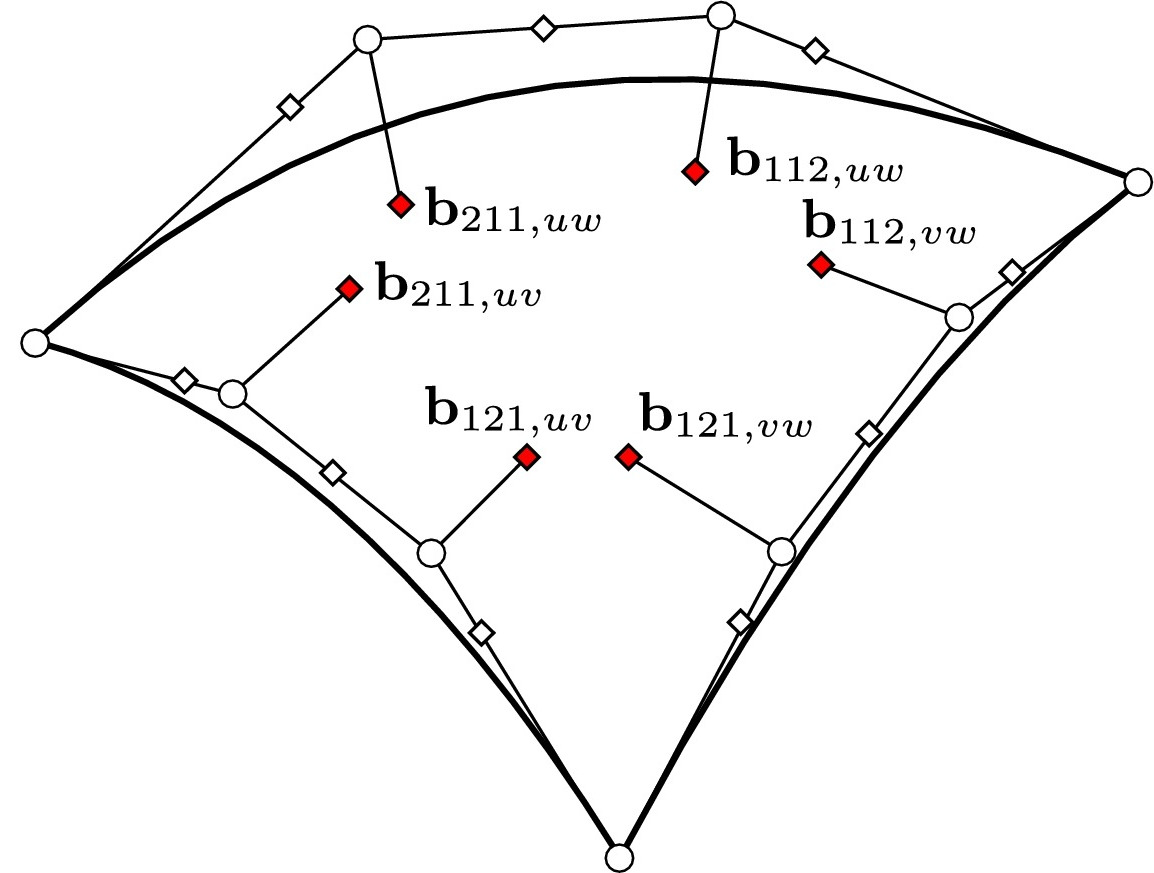
\includegraphics[width=10cm]{gregory_krpe_trikotna.jpg}
		\caption{Trikotna Gregoryjeva krpa}
	\end{figure}
\end{frame}

\section{Primeri}
\begin{frame}
	\begin{figure}[h]
		\centering
		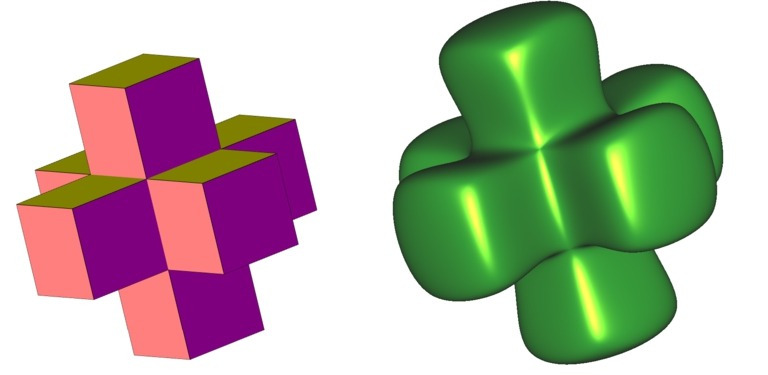
\includegraphics[width=10cm]{posebna_kocka.jpg}
	\end{figure}
\end{frame}

\begin{frame}
	\begin{figure}[h]
		\centering
		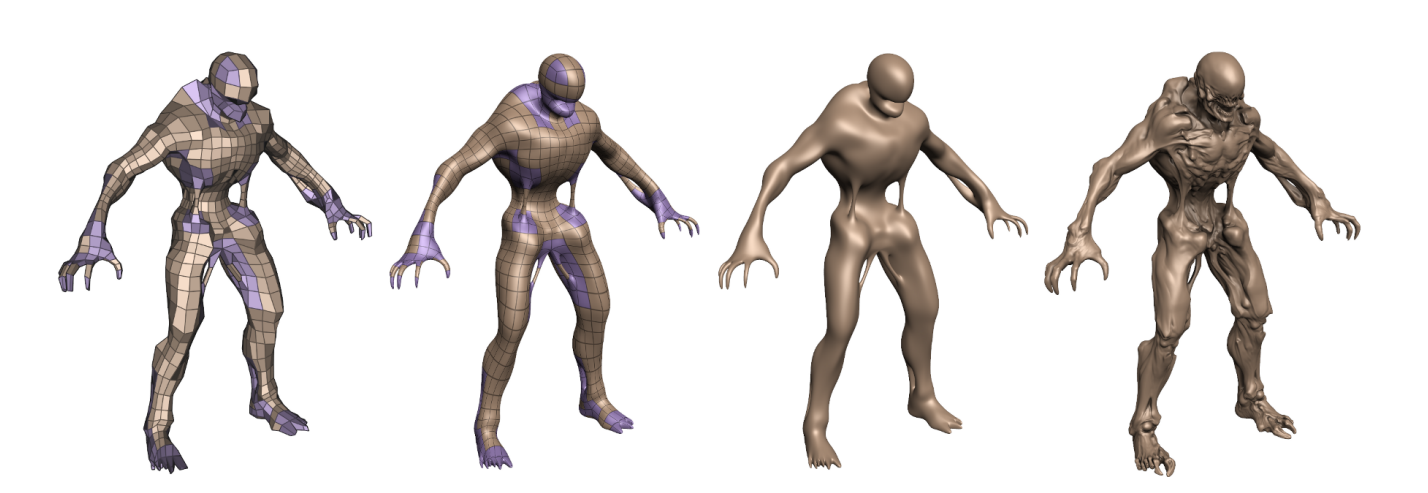
\includegraphics[width=11cm]{koncni_primer.png}
	\end{figure}
\end{frame}

\end{document}
